%%%%%%%%%%%%%%%%%%%%%%%%%%%%%%%%%%%%%%%%%%%%%%
\section{Beam requirements}
\label{sec:beamrequirements}

The requested beam parameters are driven by the requirement that the results from the CERN test beam should be directly applicable to the future large underground single-phase LAr detector with minimal extrapolation. The CERN test beam data will be used to evaluate the detector performance, to understand the various physics systematic effects, and to provide ``neutrino-like'' data for event reconstruction studies. To satisfy the requirement, the beam parameters must span a broad range of particle spectrum that are expected in the future neutrino experiment. The particle beam composition should consist of electrons, muons, and hadron beams that are charge-selected. The expected momentum distributions for secondary particles from neutrino interactions are shown in Figure~\ref{fig:ParticleMomenta}. There is a large spread in the momentum distribution with most particles peaked near 200 MeV/c.  The desirable momentum range for ProtoDUNE-SP  is in the low momentum region. Based on the feedback and constraints from the CERN beam group, the requested beamline design allows the transport of beam particles from about 0.2 GeV/c up to 7 GeV/c. 

The maximum electron drift time in the TPC is about 2.2 ms. In order to minimize pile-up in the TPC, the planned beam rate should be around 200 Hz.  The ProtoDUNE-SP TPC has two drift volumes separated by a passive cathode plane. It is desirable to aim the particle beam such that a large fraction of the lower energy hadronic showers are mostly contained in one drift volume, thus minimizing the uncertainties from particles lost in the inactive detector materials. It is also important to be able to inject beam into the cryostat at multiple locations to study the detector response. Figure~\ref{fig:beamwindow_loc} shows the three proposed beam injection points.  The angles of the beam, w.r.t. the APA plane are 3$^\circ$ (beam \#1), 8$^\circ$ (beam \#2), and 12$^\circ$ (beam \#3). Due to engineering and safety considerations, only beam \#3 will be fully instrumented with the beam window system as described in \ref{sec:beamwindow}. The remaining two beam positions will have partial installation of the beam window system. With this configuration, beam \#3 is the primary beam where most of the physics data will be taken. 
\begin{cdrfigure}[Beam window locations]{beamwindow_loc}{Beam window locations.}
  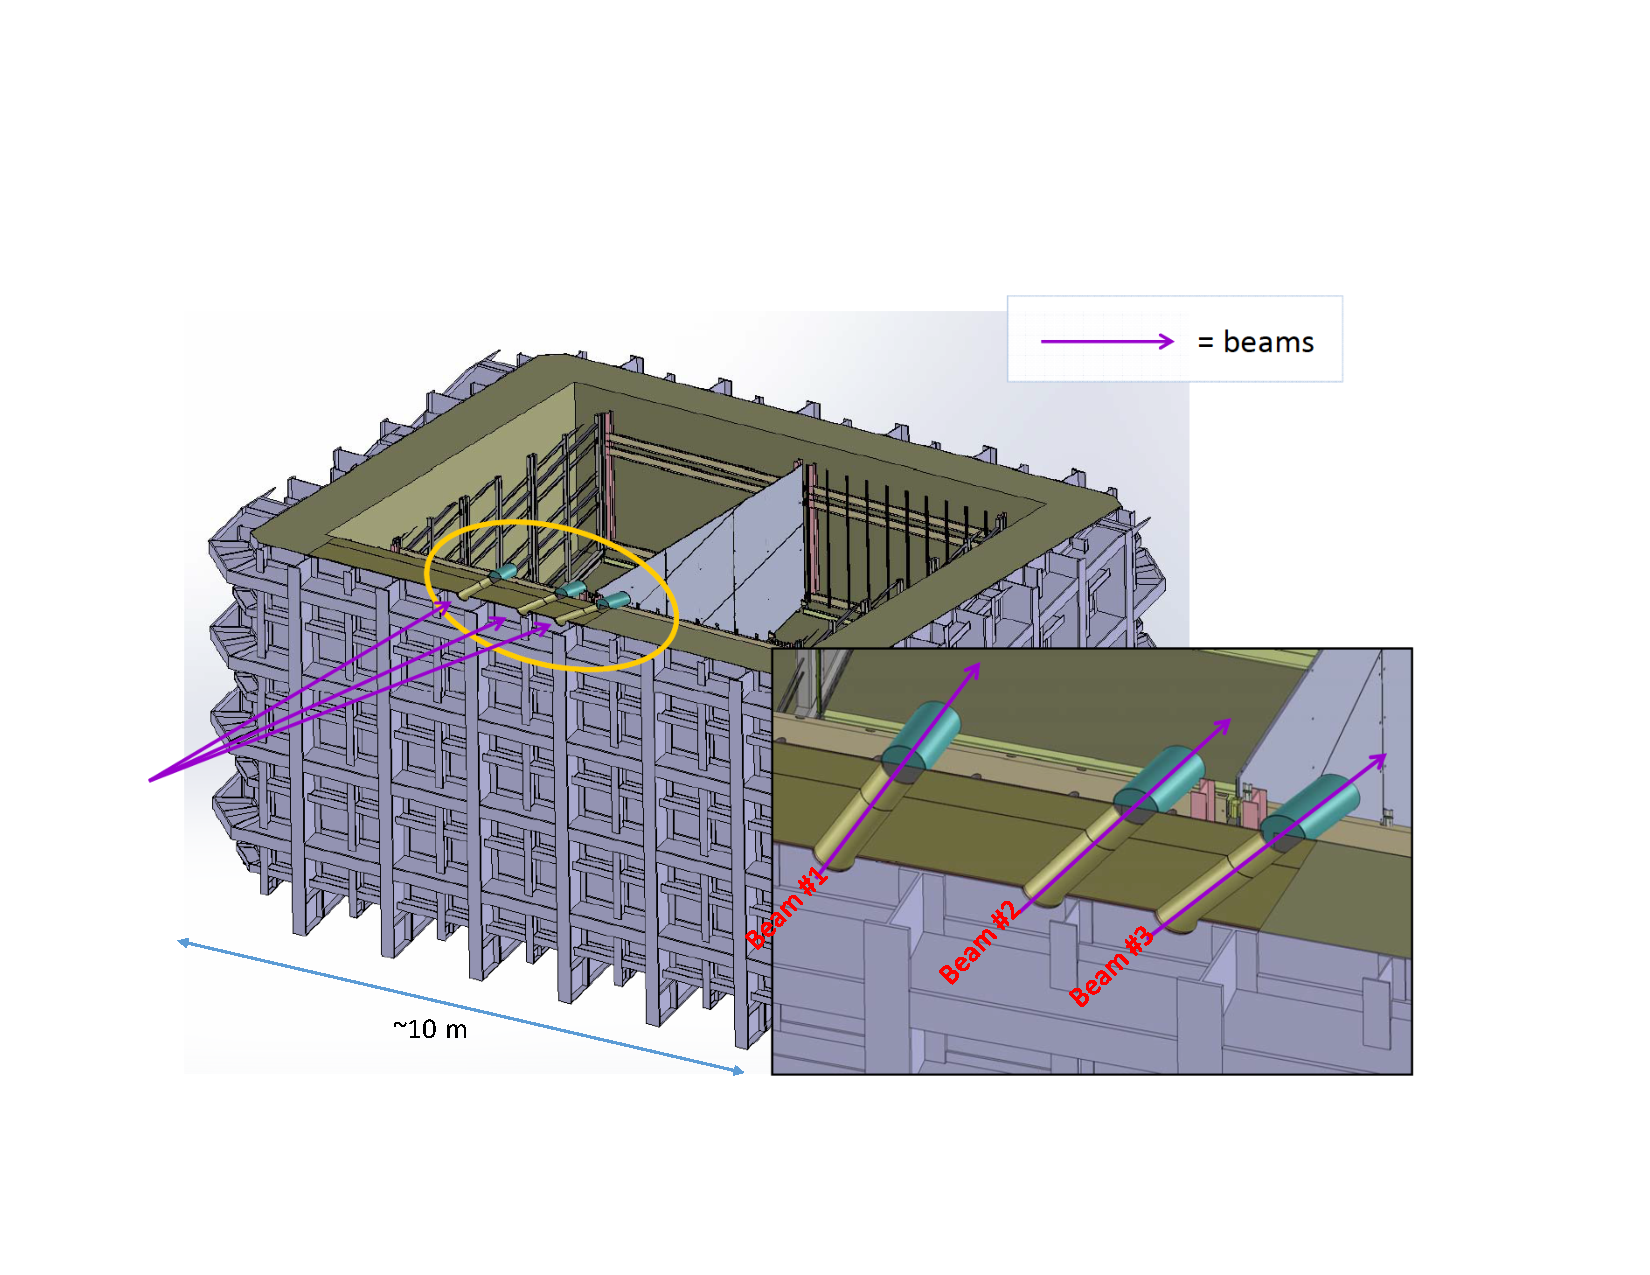
\includegraphics[width=0.9\textwidth]{beamwindow_locations.pdf}
\end{cdrfigure}
The summary of the beam requirements are shown in Table~\ref{tab:beamspecs}.
\begin{cdrtable}[Particle beam requirement]{cc}{beamspecs}{Particle beam requirements}
%\textbf{Parameter } & \textbf{Requirements}  \\ \hline
 Parameter & Requirements \\ \toprowrule
  Particle Types        & $e^\pm,\mu^\pm,\pi^\pm$,$K$,$p$  \\ \colhline
  Momentum Range   & 0.2 - 7 GeV/$c$ \\ \colhline
  Momentum Spread   & $\Delta p/p  < $5 \% \\
  & (limited by the aperture of the magnets)  \\ \colhline
  Transverse Beam Size   & RMS(x,y) $\approx$ 1 cm  \\
  & (At the entrance face of the LAr cryostat) \\ \colhline
  Beam Divergence & tbd   \\ \colhline
  Beam Entrance Position & Multiple beam windows    \\ \colhline
  Rates & 200 Hz (maximum)    \\ \colhline
\end{cdrtable}

